\documentclass{article}
\usepackage[final,sglblindworkshop]{neurips_2026}
\workshoptitle{Predictive AI Evaluation Competition}
\usepackage[T1]{fontenc}
\renewcommand{\ttdefault}{lmtt}
\usepackage[utf8]{inputenc}
\usepackage{amsmath,amssymb,booktabs,graphicx,array,tabularx,multirow}
\usepackage{float}
\usepackage{microtype}
\usepackage{xcolor}
\usepackage{url}
\usepackage{hyperref}
\usepackage{tikz}
\usetikzlibrary{arrows.meta,positioning,calc}
\hypersetup{colorlinks=true,linkcolor=blue!45!black,citecolor=blue!45!black,urlcolor=blue!45!black,pdftitle={From Overall Ability to Item-Sensitive Adaptation: Rasch-CAIMIRA for Predictive Evaluation},pdfauthor={Ankit Aggarwal and Maharshi Gor}}
\newcommand{\sigmoid}{\operatorname{sigmoid}}
\newcommand{\softmax}{\operatorname{softmax}}
\newcommand{\logit}{\operatorname{logit}}
\newcommand{\clip}{\operatorname{clip}}
\newcommand{\R}{\mathbb{R}}
\newcommand{\E}{\mathbb{E}}
\newcommand{\modelname}{Rasch--CAIMIRA}
\newcommand{\releaseurl}{https://github.com/ankaggarwal94/paiec-2026-rasch-caimira}
\newcommand{\code}[1]{\texttt{#1}}
\newcommand{\draftgap}[1]{\textbf{Draft evidence gap.} #1}
\definecolor{reportblue}{HTML}{21618C}
\definecolor{reportorange}{HTML}{B66124}
\setlength{\emergencystretch}{1.5em}
\setlength{\textfloatsep}{10pt plus 2pt minus 2pt}
\setlength{\floatsep}{9pt plus 2pt minus 2pt}
\setlength{\intextsep}{10pt plus 2pt minus 2pt}
\title{From Overall Ability to Item-Sensitive Adaptation:\\Rasch--CAIMIRA for Predictive Evaluation}
\author{Ankit Aggarwal\\Stanford University \And Maharshi Gor\\University of Maryland}
\date{}
\begin{document}
\maketitle
\begin{abstract}
A handful of observed responses can sharpen forecasts of an AI system's future performance. We present \modelname{}, a compact evaluator that combines two complementary views of adaptation. A Rasch branch updates the system's overall ability; a two-dimensional CAIMIRA-style branch determines how the update transfers across items. Both start from item text and subject metadata, and their probabilities receive equal weight. The CAIMIRA update decomposes into a shared shift and a content-dependent contrast, making the route from revealed evidence to new forecasts explicit. Our selected PAIEC candidate, \code{18-s44-rasch-caimira.zip}, achieves formative Brier area under the learning curve of \textbf{0.160822}. Across nine subject--benchmark pairs, mean Brier error falls from 0.212061 with zero labels to 0.126671 with 31 labels, a \textbf{40.27\% reduction}. Every pair improves at the final budget, and seven labels capture 76.20\% of the observed endpoint gain. The archive contains 3,076 fitted coefficients and runs with local CPU computation. We explain its adaptation geometry, analyze the complete learning curve, and develop hierarchical evidence sharing and calibrated gating as complementary extensions.
\end{abstract}

\section{Introduction}
Predictive evaluation turns a small evaluation budget into forecasts for a much larger set of items. Rather than treating a subject's observed accuracy as the final answer, it asks how each revealed outcome changes the probability of success on further questions. This creates a useful division of labor: item text and system metadata describe the problem before any labels arrive, while observed responses adapt that description to the current subject and benchmark~\citep{paiec2026}.

The central conceptual step in our design is to treat adaptation at two scales. A response can revise a subject's \emph{overall level}, and it can revise the \emph{profile of ability} that matters for a particular item. The Rasch branch estimates a shared scalar correction. The CAIMIRA-style branch estimates both a shared shift and an item-dependent contrast through two ability coordinates and item-specific relevance weights. Together, these views explain how evidence from one item changes the forecast for another.

This perspective joins the stability of classical item-response modeling~\citep{rasch1960} with CAIMIRA's content-dependent difficulty and relevance~\citep{gor2024}. A fixed lexical representation keeps the fitted model compact~\citep{weinberger2009}. At evaluation time, only the subject's ability is updated. The item model stays fixed, so each new label has a precise route into later predictions. Figure~\ref{fig:overview} shows this computation.

\paragraph{Contributions.}
First, we give a concrete formulation of global and item-sensitive adaptation in one deployable evaluator. Second, we show that the selected candidate converts sparse feedback into substantial probability-accuracy gains: every evaluated pair improves from zero to 31 labels, with most of the aggregate gain available after seven. Third, we connect the model's transparent update rule to a practical extension based on shared item structure, subject regression, and calibrated gating.


\clearpage
\section{Predictive evaluation with a small label budget}
\label{sec:task}
\paragraph{Prediction unit.}
Let $s$ describe an AI system under a fixed configuration, and let $i$ denote an item. A response is binary, $y\in\{0,1\}$. The evaluator returns $p(y=1\mid s,i,\mathcal{D}_n)$, where $\mathcal{D}_n$ contains up to $n$ revealed outcomes from the current subject--benchmark pair. Subject attributes include model name, provider, dates, harness, harness version, reasoning effort, and extra settings. The candidate serializes the entire supplied subject dictionary. For items, its predictive features use \code{item\_content}; \code{benchmark\_id} controls which support labels are eligible~\citep{release}.

\paragraph{Budgeted evaluation.}
The official protocol separates acquisition items from evaluated items and supplies nested evidence at budgets $\{0,1,3,7,15,31\}$. All six checkpoints within a submission evaluate the same response set. This archive omits \code{labeling.py}, so the platform supplies random acquisition. Formative submissions draw fresh hidden subsets; comparisons between separately submitted candidates therefore involve sample variation~\citep{paiec2026}.

\paragraph{Primary metric.}
For pair $j$, let $\mathcal{E}_j$ contain its evaluated responses, including repeated recorded responses where present. Its Brier error at budget $n$ is
\begin{equation}
 B_{j,n}=\frac{1}{|\mathcal{E}_j|}\sum_{r\in\mathcal{E}_j}(p_{j,n,r}-y_{j,r})^2.
 \label{eq:brier}
\end{equation}
The budget transformation $x=\log_2(n+1)$ places the six checkpoints at $0,1,2,3,4,5$. Trapezoidal integration over this axis, divided by its width, gives
\begin{equation}
 A_j=0.1B_{j,0}+0.2B_{j,1}+0.2B_{j,3}+0.2B_{j,7}+0.2B_{j,15}+0.1B_{j,31}.
 \label{eq:alc}
\end{equation}
The competition score is the equal-weight pair mean $J^{-1}\sum_j A_j$. Thus a small pair and a large pair have the same influence. The weights also give early adaptation substantial value: checkpoints through seven labels carry 70\% of the total weight. Brier error measures probability accuracy, with smaller values preferred; fixed $p=0.5$ yields 0.25 for every binary response~\citep{brier1950,paiec2026}.

\begin{figure}[H]
\centering
\resizebox{\linewidth}{!}{%
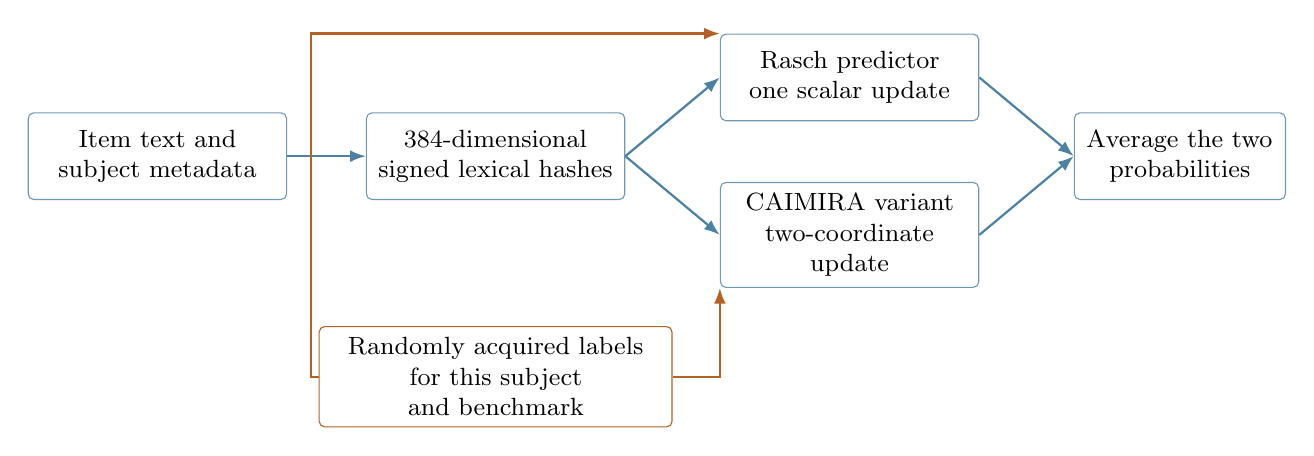
\begin{tikzpicture}[font=\small,box/.style={draw=reportblue!65,rounded corners=2pt,align=center,minimum height=11mm,text width=30mm,inner sep=4pt},arr/.style={-{Latex[length=2mm]},thick,draw=reportblue!80}]
\node[box] (attrs) {Item text and\\subject metadata};
\node[box,right=10mm of attrs] (features) {384-dimensional\\signed lexical hashes};
\node[box,right=12mm of features,yshift=10mm] (rasch) {Rasch predictor\\one scalar update};
\node[box,right=12mm of features,yshift=-10mm] (caimira) {CAIMIRA variant\\two-coordinate update};
\node[box,right=12mm of rasch,yshift=-10mm,text width=24mm] (mean) {Average the two\\probabilities};
\node[box,below=16mm of features,text width=42mm,draw=reportorange] (support) {Randomly acquired labels\\for this subject and benchmark};
\draw[arr] (attrs)--(features);
\draw[arr] (features.east)--(rasch.west);
\draw[arr] (features.east)--(caimira.west);
\draw[arr] (rasch.east)--(mean.west);
\draw[arr] (caimira.east)--(mean.west);
\draw[arr,draw=reportorange] (support.east)-|(caimira.south west);
\draw[arr,draw=reportorange] (support.west)-|([xshift=-7mm]features.west)|-(rasch.north west);
\end{tikzpicture}}
\caption{The submitted evaluator. Frozen parameters map attributes to difficulty, relevance, and ability priors. Revealed labels update a scalar offset or a two-dimensional ability vector. The final operation averages probabilities. Orange arrows indicate evidence used for adaptation.}
\label{fig:overview}
\end{figure}

\paragraph{Evaluation population.}
The formative tables cover nine subjects, seven anonymous benchmarks, and 496 distinct evaluated subject--item pairs~\citep{release}. Repeated recorded responses can make the response denominator larger than the distinct-item count. We retain the official equal-weight pair aggregation throughout the main results, giving each evaluated system--task combination the same influence.

\paragraph{A clean adaptation experiment.}
All six checkpoints reuse the same evaluation responses, so changes along a submission's curve directly describe what happens as additional support arrives. A frozen-prediction reference holds the zero-label forecast constant at every later budget. Comparing the observed curve with this reference isolates the value of using revealed evidence within this run. The larger archived replay supplies a separate comparison among the two branches and their blend.

\clearpage
\section{Two complementary views of ability}
\label{sec:models}
\paragraph{A common lexical encoder.}
The encoder case-folds text, extracts words and individual punctuation tokens using \code{\textbackslash w+|[\textasciicircum\textbackslash w\textbackslash s]}, and counts occurrences. Each token receives a deterministic signed bucket through BLAKE2b, with an eight-byte digest and personalization string \code{roadmap.lex.v1}. The first four digest bytes select one of 384 coordinates; a bit in the fifth byte selects the sign. The resulting vector is normalized to unit Euclidean length, with an all-zero vector for empty token input. This is a fixed feature map, without a fitted vocabulary~\citep{release,weinberger2009}.

Write $x_i\in\R^{384}$ for item features and $z_s\in\R^{384}$ for features of the subject dictionary's canonical JSON string. Canonical serialization sorts keys and uses compact separators. Each branch learns item effects and a prior ability from these features. Frozen forward computations use CPU tensors in float32; adaptation uses float64 arrays. Both states retain centering constants. The formulas below apply to nonzero metadata features; an all-zero vector receives prior ability zero.

\subsection{Rasch branch: one overall ability dimension}
The Rasch model assigns each item a difficulty and each subject an initial ability:
\begin{equation}
 d_i^{R}=x_i^\top w_d^{R}-c_d^{R},\qquad
 \mu_s^{R}=(z_s-\bar z^{R})^\top w_\mu^{R},\qquad
 \eta_{si}^{R}=b_R+\mu_s^{R}-d_i^{R}.
 \label{eq:rasch}
\end{equation}
The initial probability is $\sigmoid(\eta_{si}^{R})$. Every item shares the same slope with respect to ability, so increasing ability shifts every item's log odds by the same amount. The metadata map gives a prior for a subject from its attributes, rather than requiring a subject-index lookup. The state includes 769 fitted coefficients: one intercept and two 384-dimensional weight vectors~\citep{release}.

\subsection{CAIMIRA-style branch: two ability coordinates}
For two latent coordinates, the second branch computes a difficulty vector and relevance weights:
\begin{align}
 d_i^{C}&=x_i^\top W_d^{C}-c_d^{C}, &
 r_i&=\softmax(x_i^\top W_r+c_r), \\
 \mu_s^{C}&=(z_s-\bar z^{C})^\top W_\mu^{C}, &
 \eta_{si}^{C}(a)&=b_C+r_i^\top(a-d_i^{C}).
 \label{eq:caimira}
\end{align}
Here $r_i\in\R^2$ has positive entries that sum to one. An item can emphasize one ability coordinate or distribute its relevance across both. At zero labels, $a=\mu_s^{C}$. This follows CAIMIRA's content-dependent relevance and difficulty idea~\citep{gor2024}; the candidate instantiates it with lexical hashes, a learned metadata prior, rank two, and a Gaussian-prior update. Those implementation choices define the variant studied here.

\begin{table}[H]
\centering
\caption{Active components of the submitted artifact. Counts exclude frozen centering constants.}
\label{tab:implementation}
\small
\begin{tabular}{@{}lcc@{}}
\toprule
Property & Rasch branch & CAIMIRA-style branch \\
\midrule
Item / metadata feature width & 384 / 384 & 384 / 384 \\
Latent ability dimension & 1 & 2 \\
Fitted coefficient count & 769 & 2,307 \\
Adaptation & Scalar MAP offset & Native ability MAP \\
Prior precision for adaptation & 1 & Identity matrix \\
Prediction mixture weight & 0.5 & 0.5 \\
State-declared ridge setting & 0.01 & 0.01 \\
\bottomrule
\end{tabular}
\end{table}

\paragraph{What the two coordinates mean.}
These coordinates are fitted directions of ability, and each item's relevance weights determine its position between them. This gives the model a direct mechanism for transferring evidence selectively. Items with similar relevance profiles receive similar ability corrections, while items emphasizing different coordinates can respond differently to the same support set. The scalar branch supplies a complementary global correction. Together, the branches use a common input representation while expressing two distinct assumptions about transfer.

\clearpage
\section{Updating from a small set of labels}
\label{sec:adaptation}
The exported predictor first filters revealed evidence to entries whose complete subject dictionary equals the query subject and whose nonempty benchmark identifier matches the query benchmark. Only this filtered prefix enters either branch. Missing benchmark identifiers lead to zero-label predictions. Consequently, adaptation has a clear meaning: it learns from the current subject's performance on other items in the same benchmark~\citep{release}.

\subsection{A scalar correction for Rasch}
For support logits $\ell_k$ and outcomes $y_k$, the Rasch branch solves
\begin{equation}
 \hat\delta=\arg\min_{\delta\in\R}
 \left\{\frac{\delta^2}{2}+\sum_{k=1}^{n}
 \big[\log(1+e^{\ell_k+\delta})-y_k(\ell_k+\delta)\big]\right\}.
 \label{eq:offset}
\end{equation}
Its prediction becomes $p_R=\sigmoid(\ell_{\rm query}+\hat\delta)$. The zero-mean, unit-variance Gaussian prior shrinks the correction toward the initial forecast. Before this update, the implementation clips frozen probabilities to $[10^{-9},1-10^{-9}]$ and converts them to logits. The zero-label path directly returns the frozen forecast.

The derivative is $g(\delta)=\delta+\sum_k\sigmoid(\ell_k+\delta)-\sum_k y_k$. Since
\begin{equation}
 g'(\delta)=1+\sum_k p_k(\delta)[1-p_k(\delta)]>0,
\end{equation}
the objective has one minimizer. The derivative has the required opposite signs at $-n$ and $n$, giving a bracket for a deterministic solver. The source performs 42 bisection steps. In exact arithmetic, the final midpoint is within $n/2^{42}$ of the root. Thus the scalar update has a transparent numerical target even with unanimous support labels.

\subsection{A two-coordinate correction for CAIMIRA}
Write $o_k=b_C-r_k^\top d_k^C$. The CAIMIRA-style branch solves
\begin{equation}
 \hat a=\arg\min_{a\in\R^2}
 \left\{\frac{1}{2}\|a-\mu_s^C\|_2^2+
 \sum_{k=1}^{n}\big[\log(1+e^{o_k+r_k^\top a})-y_k(o_k+r_k^\top a)\big]\right\},
 \label{eq:native}
\end{equation}
then returns $p_C=\sigmoid(b_C+r_i^\top[\hat a-d_i^C])$. The Hessian is
$I+\sum_k p_k(1-p_k)r_kr_k^\top$, which is positive definite. Frozen item parameters and a quadratic prior therefore produce a unique posterior mode. The implementation uses SciPy L-BFGS-B with an analytic gradient, initializing at the metadata prior. It rejects nonfinite objectives and failed solves whose largest absolute gradient component exceeds $10^{-6}$.

\paragraph{The geometry of item-sensitive adaptation.}
The two-coordinate update admits an especially simple interpretation. Let $u=\hat a-\mu_s^C$, $\bar u=(u_1+u_2)/2$, and $v=(u_1-u_2)/2$. Because $r_{i1}+r_{i2}=1$, its change in log odds is exactly
\begin{equation}
 r_i^\top u=\bar u+(r_{i1}-r_{i2})v.
 \label{eq:geometry}
\end{equation}
The first term shifts every item together. The second adds a content-dependent contrast. Thus even two coordinates create a meaningful extension of scalar adaptation: evidence can change both the subject's overall level and its relative performance across item profiles. This is the conceptual core of the model.

\subsection{Probability averaging}
The final predictor is $p=(p_R+p_C)/2$. For any binary outcome $y$,
\begin{equation}
 (p-y)^2=\tfrac12(p_R-y)^2+\tfrac12(p_C-y)^2-\tfrac14(p_R-p_C)^2.
 \label{eq:mixture}
\end{equation}
Under the Brier objective, disagreement contributes a precisely quantified reduction relative to the mean component loss. Equal weights preserve both adaptation views without introducing an additional fitted combiner. Section~\ref{sec:calibration} measures the blend against each branch on a common archived panel; Section~\ref{sec:extensions} describes how a learned gate could extend this fixed combination.

\clearpage
\section{Results: strong gains from sparse feedback}
\label{sec:results}
Submission 1033935 is associated with the attached archive through the submission ledger's exact SHA-256 and byte count. The supplied screenshot reports a completed run and Brier ALC of 0.160822~\citep{release}. Averaging its nine displayed pair ALCs reproduces 0.160822 exactly. Applying Equation~\ref{eq:alc} to the rounded per-budget rows gives 0.160821878, a difference consistent with six-decimal reporting. This reconciliation connects the screenshot, pair summary, and complete learning curve.

\begin{figure}[H]
\centering
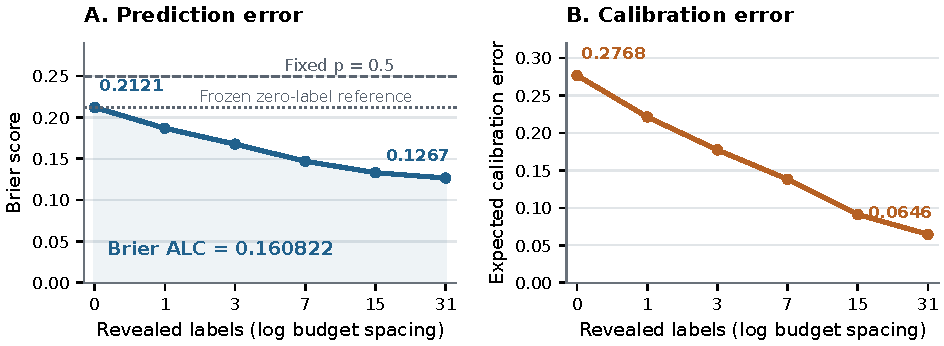
\includegraphics[width=\linewidth]{figures/learning_curves.pdf}
\caption{Pair macro means from the supplied scoring tables. The Brier curve improves at every checkpoint. The dotted reference freezes each target's zero-label prediction at all later budgets; the dashed reference always predicts 0.5. The shaded area represents the normalized learning-curve calculation up to its constant axis-width factor. ECE is a separate calibration diagnostic.}
\label{fig:macro}
\end{figure}

\begin{table}[H]
\centering
\caption{Aggregate results. Each row averages the same nine subject--benchmark pairs equally.}
\label{tab:budget}
\small
\begin{tabular}{@{}rrrrr@{}}
\toprule
Labels & ALC weight & Mean Brier & Mean ECE & Brier gain from zero \\
\midrule
0  & 0.10 & 0.212061 & 0.276844 & 0.000000 \\
1  & 0.20 & 0.186937 & 0.221364 & 0.025124 \\
3  & 0.20 & 0.167660 & 0.177372 & 0.044401 \\
7  & 0.20 & 0.146991 & 0.138118 & 0.065070 \\
15 & 0.20 & 0.133155 & 0.091226 & 0.078906 \\
31 & 0.10 & 0.126671 & 0.064634 & 0.085390 \\
\bottomrule
\end{tabular}
\end{table}

\paragraph{Magnitude of adaptation.}
Mean Brier error decreases by 0.085390 from zero to 31 labels, or 40.27\% relative to the zero-label value. Seven labels capture 76.20\% of that observed endpoint gain; fifteen capture 92.41\%. The first few responses therefore carry substantial practical value. Later checkpoints continue to improve the average, with diminishing mean reduction per additional label.

\paragraph{Two transparent references.}
The fixed-0.5 reference has Brier ALC 0.25, so the ensemble's reported ALC is 35.67\% lower. This is an arithmetic reference that requires only binary outcomes. A second reference holds each target's initial prediction fixed throughout evaluation. Its learning curve is flat at the observed zero-label Brier mean, 0.212061. Against that reference, observed adaptation reduces ALC by 0.051239, or 24.16\%. These transparent references quantify the value of the forecast and its adaptation using the same recorded response set.

\paragraph{Aggregation matters.}
Weighting the nine pair ALCs by their displayed distinct-item counts instead gives 0.159046. That diagnostic changes the weighting rule and differs from the official score. We consistently report the equal-weight pair mean. We also preserve the distinction between 496 unique subject--item pairs and the response-level denominator used inside each pair's Brier calculation.

\clearpage
\section{Adaptation gains across evaluated pairs}
\label{sec:heterogeneity}
The pair-level curves reveal how broadly the aggregate gain extends. Figure~\ref{fig:pairs} gives each pair the same axes and retains the anonymous identifiers supplied by the scorer. Every pair finishes below its own zero-label Brier error. The magnitude varies substantially: pair ALC ranges from 0.068828 to 0.246809. Six pairs have at least one intermediate increase, accounting for eight of the 45 adjacent transitions, while the final-budget gain is shared by all nine.

\begin{figure}[H]
\centering
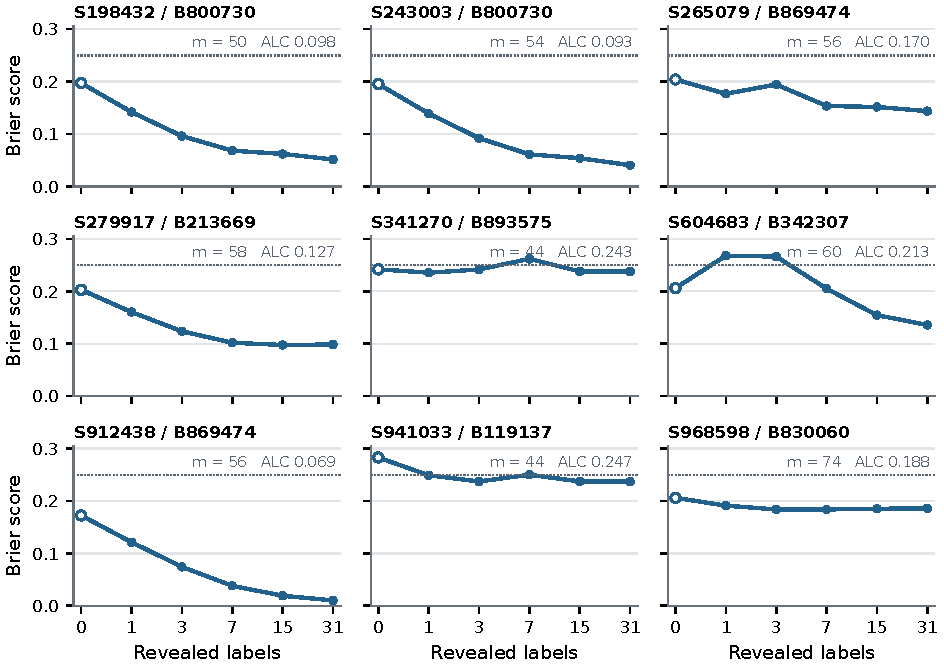
\includegraphics[width=.98\linewidth]{figures/pair_learning_curves.pdf}
\caption{All nine pair learning curves, with a common Brier scale. S and B abbreviate the published anonymous subject and benchmark prefixes; $m$ is the number of distinct evaluated subject--item pairs. Open markers show the initial forecast. Dotted lines show the fixed-0.5 reference. The horizontal positions use the same logarithmic budget transformation as Figure~\ref{fig:macro}.}
\label{fig:pairs}
\end{figure}

\begin{table}[H]
\centering
\caption{Pair-level results. Gain is $B_0-B_{31}$; larger values indicate more improvement.}
\label{tab:pairs}
\small
\begin{tabular}{@{}llrrrr@{}}
\toprule
Subject & Benchmark & $m$ & ALC & $B_{31}$ & Gain \\
\midrule
198432 & 800730 & 50 & 0.098321 & 0.051231 & 0.145805 \\
243003 & 800730 & 54 & 0.092645 & 0.040327 & 0.154904 \\
265079 & 869474 & 56 & 0.169868 & 0.143456 & 0.060445 \\
279917 & 213669 & 58 & 0.126733 & 0.098363 & 0.104464 \\
341270 & 893575 & 44 & 0.243301 & 0.237775 & 0.004090 \\
604683 & 342307 & 60 & 0.212877 & 0.135660 & 0.070355 \\
912438 & 869474 & 56 & 0.068828 & 0.010232 & 0.162210 \\
941033 & 119137 & 44 & 0.246809 & 0.237130 & 0.045958 \\
968598 & 830060 & 74 & 0.188016 & 0.185867 & 0.020278 \\
\bottomrule
\end{tabular}
\end{table}

\paragraph{Three useful patterns.}
S912438 shows how strongly a small support set can sharpen a forecast: its Brier error falls from 0.172442 to 0.010232, a 94.07\% reduction. S604683 illustrates recovery as evidence accumulates: error rises to 0.267988 after one label, then falls to 0.135660 by the final budget. S341270 has a modest gain of 0.004090, identifying a setting where richer item structure could be valuable. Together, these trajectories suggest a practical development strategy: preserve rapid adaptation where it succeeds and target additional modeling capacity at the flatter curves.

\clearpage
\section{Calibration and component evidence}
\label{sec:calibration}
\paragraph{Accuracy and calibration improve together.}
Expected calibration error (ECE) compares predicted probabilities with response frequencies in ten equal-width bins, weighted by response count~\citep{paiec2026}. In the formative feedback, pair macro ECE falls from 0.276844 at zero labels to 0.064634 at 31 labels, a 76.65\% reduction. Its budget-weighted macro value is approximately 0.159763.

\begin{figure}[H]
\centering
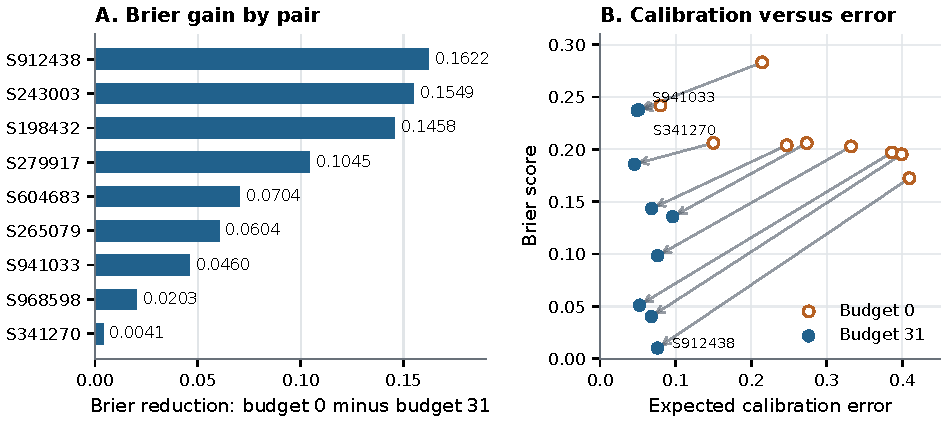
\includegraphics[width=.96\linewidth]{figures/adaptation_calibration.pdf}
\caption{Two complementary views of the formative run. Left: absolute Brier improvement from zero to 31 labels. Right: arrows connect each pair's initial and final ECE--Brier coordinates. Each pair improves in endpoint Brier error; the joint view shows how probability accuracy and calibration change together.}
\label{fig:calibration}
\end{figure}

The two measures also help identify the next modeling opportunity. For S941033, ECE at fifteen labels is 0.015630 while Brier error is 0.237347. Matching an overall response frequency can still leave room to distinguish easier and harder items. We therefore use Brier error as the primary measure and ECE as a complementary diagnostic.

\paragraph{A common-panel component comparison.}
An archived replay evaluated the exact candidate on 153 subject--benchmark pairs across 30 public benchmarks and 21,788 evaluation response rows. The protocol uses the same item split, acquisition stream, and evaluation set across packages~\citep{release}. Table~\ref{tab:local} isolates the recorded results for the Rasch branch, CAIMIRA-style branch, and equal blend.

\begin{table}[H]
\centering
\caption{Archived component replay; lower is better. Three sources (25 pairs) also occur in CAIMIRA training.}
\label{tab:local}
\small
\begin{tabular}{@{}lrrr@{}}
\toprule
Package & Brier ALC & ECE ALC & Brier difference vs. Rasch \\
\midrule
Rasch offset (16) & 0.200183 & 0.150166 & 0.000000 \\
Equal blend (18) & 0.201449 & 0.153118 & +0.001267 \\
CAIMIRA-style native (27) & 0.202985 & 0.156827 & +0.002803 \\
\bottomrule
\end{tabular}
\end{table}

The blend improves on CAIMIRA alone by 0.001536 ALC and on the mean component loss by 0.000135, consistent with Equation~\ref{eq:mixture}. Rasch alone has the strongest point estimate, leading the blend by 0.001267. The two views of adaptation are therefore close in this replay, with equal averaging providing a transparent combination and learned weighting offering a focused next step.

\paragraph{Evidence scope and limitations.}
The formative evaluation establishes a within-run adaptation gain. The local replay uses one seed and label-informed pair selection; 25 pairs share sources with CAIMIRA training. It serves as a component diagnostic. Appendix~\ref{app:training} documents the 44-benchmark CAIMIRA fit; the exact Rasch fitting receipt remains \textbf{UNVERIFIED}. Source-separated comparisons would assess transfer more directly. Appendix~\ref{app:reproduction} describes fresh CPU execution and reproduction.

\clearpage
\section{Extension: shared evidence and calibrated gating}
\label{sec:extensions}
The selected Rasch--CAIMIRA candidate adapts within one subject--benchmark pair. A complementary hierarchical IRT line, developed in an earlier internal study and implemented in \code{submit\_gate.zip}, makes each revealed label useful more broadly~\citep{release}. It connects related items and subjects and calibrates two variants of online inference. This extends our two-scale adaptation view through shared evidence.

\subsection{Sharing evidence through item and subject structure}
The hierarchical model starts from a conditional ability-minus-difficulty relation,
\begin{equation}
 \logit p_{s,i}^{\rm cond}=\beta_b+\delta_{s,b}-d_i,
 \qquad
 d_i=\widehat d_i+q_i^\top v_b+\sum_k a_{ik}g_{b,k}+\epsilon_i.
 \label{eq:hierarchical}
\end{equation}
Here $p_{s,i}^{\rm cond}$ conditions on the latent effects, $\widehat d_i$ is a frozen content prior, $q_i$ is a 64-dimensional projected item representation, $g_{b,k}$ denotes shared item-group effects, and $\epsilon_i$ is an item-specific residual. Items can share groups through key-value metadata or identical content. A label can therefore update both the observed item and related items on the same benchmark.

Subject ability has the form $\delta_{s,b}=h_s^\top w_b+r_{s,b}$, where $h_s$ contains subject descriptors and frozen ability summaries, $w_b$ is a benchmark-specific regression, and $r_{s,b}$ is a subject residual. Revealed outcomes from several subjects can improve that shared regression. This supplies a different source of transfer from CAIMIRA's item-relevance geometry: one learns where an ability update matters, while the other pools evidence across related observations.

\subsection{Calibrating the strength of online updates}
The gate package combines two members built from the same offline fit. One uses variance-adjusted likelihood updates, denoted $p_{\rm VI}$; the other uses MAP-style likelihood updates, denoted $p_{\rm MAP}$. Both marginalize variance in their final probability calculation. Writing $p_{\rm VI}$ and $p_{\rm MAP}$ for their probabilities clipped to $[10^{-4},1-10^{-4}]$, the stored gate at $n$ labels is approximately
\begin{equation}
 p_G=
 \begin{cases}
 p_{\rm VI}, & n=0,\\
 \sigmoid\!\left(2.3581\logit p_{\rm VI}-1.7053\logit p_{\rm MAP}\right), & n\ge1.
 \end{cases}
 \label{eq:gate}
\end{equation}
The negative coefficient makes this a signed calibration in log-odds space. It can adjust the strength of adaptation beyond an average of the two member probabilities. Appendix~\ref{app:gate} traces the implementation. On a separate 20-benchmark protocol, the earlier study records Gate ALC 0.2077 versus 0.2202 for its base IRT model, motivating this extension; Appendix~\ref{app:shared} preserves that study and its evaluation scope.

\subsection{A concrete composition to evaluate}
A simple candidate for joining the systems is
\begin{equation}
 p_{\rm ext}=\tfrac12p_{RC}+\tfrac12p_G
            =\tfrac14p_R+\tfrac14p_C+\tfrac12p_G,
 \qquad p_{RC}=\tfrac12(p_R+p_C).
 \label{eq:extension}
\end{equation}
This proposal preserves both selected branches and adds the hierarchical model as a complementary forecast. A budget-dependent weight is a further option once matched replay data are available. The combined predictor's empirical benefit remains a question for the next experiment.

A useful comparison would fix panel, support prefixes, and evaluation responses across Rasch, CAIMIRA, the selected blend, the gate, and Equation~\ref{eq:extension}, then repeat across acquisition seeds. The gate's separate uncertainty policy accepts probabilities in $[0.2,0.8]$ with a budget-fill rule. Evaluating that policy in a second stage would distinguish gains from prediction and label selection.

\paragraph{Conclusion.}
Rasch--CAIMIRA makes sparse predictive evaluation concrete: use a stable global correction, add item-sensitive adaptation, and combine their forecasts in a compact package. The selected candidate reaches Brier ALC 0.160822 and reduces endpoint Brier error by 40.27\%, with most of the gain present after seven labels. Its transparent geometry provides a strong foundation for the next stage: sharing evidence across related items and subjects, and learning how strongly to trust each adaptation view.

\clearpage
\section*{Acknowledgments and disclosure}
ChatGPT assisted with artifact inspection, calculations, figure generation, exposition, and source verification. Claude Code (Anthropic) assisted with coding, testing, experiments, and the earlier hierarchical IRT manuscript. The authors retain responsibility for the scientific claims and final submission. The report describes the selected Rasch--CAIMIRA package and a separately identified hierarchical extension.

\begin{thebibliography}{9}
\bibitem[AIMS(2026a)]{paiec2026}
AIMS. \emph{The Predictive AI Evaluation Competition at NeurIPS 2026}. Competition rules, interface, and evaluation specification. \url{https://aims.stanford.edu/competition}. Accessed November 6, 2026, Pacific time.

\bibitem[Aggarwal and Gor(2026)]{release}
Ankit Aggarwal and Maharshi Gor. \emph{Rasch--CAIMIRA reproducibility package}. Code, fitted states, source manifests, and evaluation summaries accompanying this report, 2026. Companion repository: \url{https://github.com/ankaggarwal94/paiec-2026-rasch-caimira}.

\bibitem[Brier(1950)]{brier1950}
Glenn W. Brier. Verification of forecasts expressed in terms of probability. \emph{Monthly Weather Review}, 78(1):1--3, 1950. \url{https://journals.ametsoc.org/view/journals/mwre/78/1/1520-0493_1950_078_0001_vofeit_2_0_co_2.xml}.

\bibitem[Gor et~al.(2024)]{gor2024}
Maharshi Gor, Hal Daum\'{e}~III, Tianyi Zhou, and Jordan Boyd-Graber. Do great minds think alike? Investigating Human-AI Complementarity in Question Answering with CAIMIRA. In \emph{Proceedings of EMNLP}, pages 21533--21564, 2024. \url{https://aclanthology.org/2024.emnlp-main.1201/}.

\bibitem[Rasch(1960)]{rasch1960}
Georg Rasch. \emph{Probabilistic Models for Some Intelligence and Attainment Tests}. Danish Institute for Educational Research, Copenhagen, 1960.

\bibitem[AIMS(2026b)]{measurementdb2026}
AIMS. \emph{The AI Measurement Data Bank}. AIMS Lab, Stanford University, 2026. \url{https://huggingface.co/datasets/aims-foundations/measurement-db}.

\bibitem[Weinberger et~al.(2009)]{weinberger2009}
Kilian Weinberger, Anirban Dasgupta, John Langford, Alex Smola, and Josh Attenberg. Feature hashing for large scale multitask learning. In \emph{Proceedings of the 26th International Conference on Machine Learning}, pages 1113--1120, 2009. \url{https://alex.smola.org/papers/2009/Weinbergeretal09.pdf}.
\end{thebibliography}

\clearpage
\appendix
\section{Artifact identity and implementation trace}
\label{app:identity}
The source archive supplied for this draft is named \code{18-s44-rasch-caimira(1).zip}. Its ordinary SHA-256 is
\begin{center}\small\ttfamily
23546eb90c7469fe7ea2704879775885f1b32e3277b4b7b3a1015aa1c7c6297b
\end{center}
The filename suffix is local to the attachment. The archived submission ledger lists the same checksum and byte count under \code{18-s44-rasch-caimira.zip}, linking it to submission 1033935. Its recorded creation time is November 4, 2026, at 23:38:06 UTC, which corresponds to 15:38:06 Pacific Standard Time and agrees with the supplied screenshot's displayed minute.

\begin{table}[H]
\centering
\caption{Files inside the exact candidate archive.}
\begin{tabularx}{\linewidth}{@{}p{.45\linewidth}r>{\raggedright\arraybackslash}X@{}}
\toprule
File & Uncompressed bytes & Role \\
\midrule
\code{model.py} & 53,370 & Exported predictor and branch implementations \\
\code{caimira-requires-state.json} & 70,999 & Rank-two fitted state \\
\code{rasch-requires-state.json} & 35,785 & Rank-one fitted state \\
\bottomrule
\end{tabularx}
\end{table}

\begin{table}[H]
\centering
\caption{Source locations in the supplied \code{model.py}. The two setup functions contain duplicated shared machinery.}
\small
\begin{tabularx}{\linewidth}{@{}p{.39\linewidth}p{.15\linewidth}>{\raggedright\arraybackslash}X@{}}
\toprule
Claim or component & Lines & What the source establishes \\
\midrule
Selected CAIMIRA-style branch & 1--2, 533--548 & Native adaptation, CPU state loading. \\
Signed lexical representation & 21--44 & Fixed 384-wide token hashing and short-string cache. \\
Support eligibility and budget check & 89--117 & Exact subject equality, benchmark match, at most 31 labels. \\
Native MAP objective & 130--142 & Gaussian prior, logistic loss, analytic gradient. \\
Difficulty and relevance & 240--269 & Frozen-centered difficulty and softmax relevance. \\
Metadata ability prior & 287--291 & Centered metadata features mapped to ability. \\
Native predictive path & 480--511 & Support-conditioned ability estimate. \\
Selected Rasch branch & 550--551, 1082--1097 & Scalar-offset adaptation. \\
Exported mixture & 1103--1109 & Equal probability weights for the two branch calls. \\
\bottomrule
\end{tabularx}
\end{table}

\paragraph{Frozen-state details.}
Both states use schema \code{proxy-structured-inductive/v1}. They store metadata ability priors, 384-wide item and subject features, and float32 parameters. The CAIMIRA-style state's intercept is 0.00920093 and its difficulty center is $(-0.06322815,-0.28565839)$. The Rasch state's intercept is 0.02624727 and its difficulty center is $-0.30726913$. Each branch retains a 384-dimensional subject-feature center. Matrix shapes and all values remain available in the original candidate ZIP; rounded values here serve orientation only.

\paragraph{Scope of the code account.}
The packaged module includes unused support for further model families, training-related configuration names, and an empirical-mean helper. Those symbols alone provide evidence of shared source machinery. The top-level function's explicit calls identify the active computation. The report describes that active computation and keeps speculative extensions in the future-work discussion.

\paragraph{Validation performed for this revision.}
Checks cover archive integrity, the interface, source paths, state shapes, equations, and score reconstruction. CPU execution passed at all six budgets in two environments, including a fresh isolated installation. Repeat calls and fresh processes agreed exactly on synthetic fixtures; input guards and support isolation passed. Appendix~\ref{app:reproduction} gives the environment and commands. Accuracy evidence retains its historical replay scope.

\clearpage
\section{Complete scoring tables}
\label{app:fullscores}
These tables reproduce the six-decimal values in the supplied scoring output. Subject and benchmark identifiers retain their anonymous suffixes. Table~\ref{tab:pairs} maps each subject to its benchmark and distinct evaluation count. ECE values are diagnostics with a response-count denominator within each pair; the report's macro summaries then weight pairs equally.

\begin{table}[H]
\centering
\caption{Brier error at every reported label budget.}
\small
\begin{tabular}{@{}lrrrrrr@{}}
\toprule
Subject & 0 & 1 & 3 & 7 & 15 & 31 \\
\midrule
198432 & .197036 & .141744 & .095946 & .067952 & .061828 & .051231 \\
243003 & .195231 & .138863 & .091878 & .061027 & .053679 & .040327 \\
265079 & .203901 & .176585 & .194296 & .153350 & .151432 & .143456 \\
279917 & .202827 & .160266 & .123605 & .101692 & .097504 & .098363 \\
341270 & .241865 & .235420 & .241557 & .261820 & .237886 & .237775 \\
604683 & .206015 & .267988 & .266198 & .204948 & .154412 & .135660 \\
912438 & .172442 & .121322 & .074291 & .038093 & .019099 & .010232 \\
941033 & .283088 & .249099 & .237301 & .250187 & .237347 & .237130 \\
968598 & .206145 & .191146 & .183869 & .183852 & .185207 & .185867 \\
\bottomrule
\end{tabular}
\end{table}

\begin{table}[H]
\centering
\caption{Expected calibration error at every reported label budget.}
\small
\begin{tabular}{@{}lrrrrrr@{}}
\toprule
Subject & 0 & 1 & 3 & 7 & 15 & 31 \\
\midrule
198432 & .386220 & .306276 & .218805 & .140396 & .116296 & .052273 \\
243003 & .399063 & .320803 & .236614 & .158748 & .133699 & .067694 \\
265079 & .246940 & .183921 & .226751 & .104399 & .094978 & .068300 \\
279917 & .332160 & .260306 & .176277 & .095509 & .070140 & .076048 \\
341270 & .079923 & .014334 & .080866 & .165216 & .052031 & .050887 \\
604683 & .273533 & .369661 & .367233 & .271586 & .154354 & .096089 \\
912438 & .409337 & .341324 & .263773 & .183032 & .120792 & .075945 \\
941033 & .214510 & .109379 & .015256 & .114241 & .015630 & .049010 \\
968598 & .149906 & .086268 & .010770 & .009931 & .063112 & .045460 \\
\bottomrule
\end{tabular}
\end{table}

\begin{figure}[H]
\centering
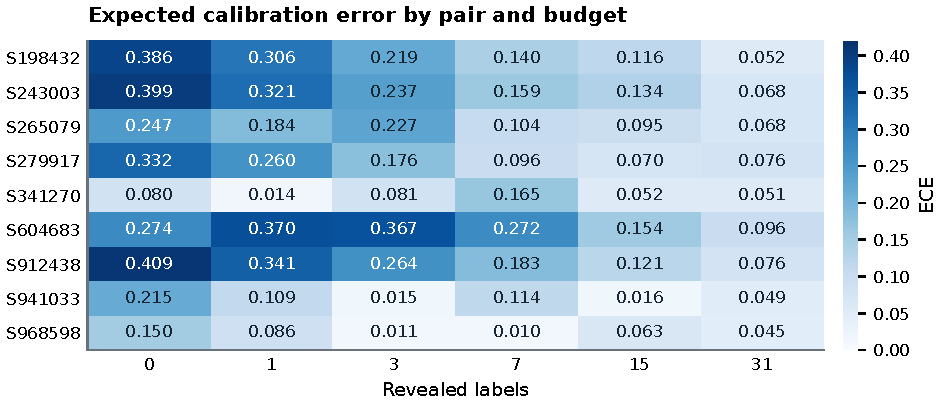
\includegraphics[width=.95\linewidth]{figures/ece_heatmap.pdf}
\caption{The complete ECE table as a heatmap. Darker cells indicate larger calibration error. A common color scale preserves comparisons across pairs and budgets.}
\end{figure}

\paragraph{Reconstruction tolerance.}
All analysis uses the supplied rounded values. Reconstructed pair ALCs differ from displayed pair summaries by at most $6\times10^{-7}$; the corresponding ECE discrepancy is at most $5\times10^{-7}$. Such differences are compatible with separately rounded inputs and summaries. The nine displayed ALC entries average exactly to the shown score of 0.160822.

\clearpage
\section{Archived local replay and protocol}
\label{app:local}
The local replay was frozen on November 5, 2026, at 03:21:03 UTC. Its manifest records Measurement Data Bank revision \code{54074453da7b9911be0f48e4c560be547bc84d21}, 153 subject--benchmark pairs, 30 benchmarks, 14,494 acquisition items, 14,492 distinct evaluation inputs, and 21,788 evaluation response rows. The 507,743,249-byte panel has SHA-256
\begin{center}\small\ttfamily
7504b6678c99873ef248027e282779c455225c721231359b76ec7a651170b116
\end{center}

\begin{table}[H]
\centering
\caption{Archived local mean Brier curves. Values are rounded from \code{summary.json}.}
\small
\begin{tabular}{@{}rrrr@{}}
\toprule
Labels & Rasch offset & Equal blend & CAIMIRA-style native \\
\midrule
0 & .250663 & .250457 & .250295 \\
1 & .226010 & .227857 & .230000 \\
3 & .199429 & .201879 & .204771 \\
7 & .185937 & .187306 & .189032 \\
15 & .177944 & .178587 & .179419 \\
31 & .172524 & .172778 & .173115 \\
\midrule
ALC & .200183 & .201449 & .202985 \\
\bottomrule
\end{tabular}
\end{table}

\paragraph{Package linkage.}
The run \code{1033935\_18-s44-rasch-caimira} records the exact candidate checksum from Appendix~\ref{app:identity}, a finished status, exit code zero, 82,734 prediction calls, 4,218 reused predictions, and 4,743 resolved support labels. The Rasch and CAIMIRA-style package receipts share the same panel and kit hashes. Their archive hashes are, respectively,
\begin{center}\small\ttfamily
7e7b3fdd2ad0343937330dc866ee29baa09ba76fb88cc1b42f4a8439ea1d3044\\
5dfbd0e6ee27b91524525618fbad0883b351b95e9c2eab3e9fc7cc8a2dafa5c0
\end{center}
An archived package audit reports identical reused structured-state bytes across these packages, with CAIMIRA and Rasch prefixes \code{348088f3} and \code{477130aa}. These match the states inspected in the supplied blend. This establishes a documented component comparison; an independent raw-prediction replay would further strengthen it.

\paragraph{Protocol and population.}
The evaluator documentation specifies item-level 50/50 acquisition/evaluation separation, a maximum of 200 items per pair, nested budgets, and a common random acquisition stream. Split and order seeds are both 20261105. Every recorded evaluation response is scored, while a single recorded response per acquired item supplies its revealed label. Pair selection is stratified using response rates. Ten benchmarks have a single admitted subject; four admit binary-valued records from a mixed-response catalog. The panel therefore has a deliberately constructed population.

\paragraph{Runtime scope.}
The blend's recorded wall time is 906.692 seconds with four prediction workers on the archived local setup. Its receipt lists Python 3.12.11, NumPy 2.5.2, SciPy 1.18.1, and PyTorch 2.13.0. These are historical local execution facts, rather than a fresh timing experiment or a hosted runtime estimate. The local panel is larger than the hosted sample, and this timing applies to the archived local environment.

\paragraph{Shared source data with CAIMIRA training.}
Three benchmarks are shared with CAIMIRA training: \code{finegrain\_t2i} (5 replay pairs), \code{medagentboard} (10), and \code{tau2\_bench} (10). Their pinned native item, response, and subject table hashes match across the manifests. The remaining 128 pairs span 27 names outside the 44-benchmark training manifest. Exact evaluated-row intersections and wider source ancestry require the materialized corpus and panel. This replay is therefore a component diagnostic; source-separated transfer requires a dedicated evaluation.

\paragraph{Verification scope.}
The manifests, protocol, receipts, summary, and package CSV agree on counts, identities, and scores. Source-overlap checks are included in the release. A sensitivity calculation on the remaining 128 pairs awaits the raw results; the aggregate values preserve the recorded 153-pair population.

\clearpage
\section{Hierarchical extension: artifact and implementation}
\label{app:gate}
The inspected extension archive is \code{submit\_gate.zip}, 190,003 bytes, with SHA-256
\begin{center}\small\ttfamily
ddb2ad28e3887324f381777aedcefd75ec22515f09144c966f5df273c80b1a31
\end{center}
Its serialized predictor selects \code{paiec.predictors.irt\_mix:IRTItemMix}. The build record lists 180 benchmarks in its build inventory and pins Measurement Data Bank revision
\begin{center}\small\ttfamily
54074453da7b9911be0f48e4c560be547bc84d21
\end{center}
These records belong to this extension archive; the selected s44 states have a separate provenance history.

\begin{table}[H]
\centering
\caption{Settings recovered from the extension package.}
\small
\begin{tabularx}{\linewidth}{@{}p{.37\linewidth}>{\raggedright\arraybackslash}X@{}}
\toprule
Component & Active setting \\
\midrule
Item features & 1,024 hash coordinates plus four dense features; lexical tokens use up to 4,000 characters, and length/style features use up to 8,000. \\
Subject features & 256 hashed dimensions plus structured descriptors. \\
Online item map & 64-dimensional seeded random projection. \\
Initial item variance allocation & Content map 0.3; key-value groups 0.2; identical-content groups 0.2; item residual 0.3. \\
Online updates & 15 iterations; empirical-Bayes scale adjustments with pseudo-count 10. \\
Subject regression & Benchmark-local shared weights and subject residuals; \code{subject\_sharing=false}. \\
Gate members & Same offline fit, subject regression enabled; \code{vi=true, vi\_frac=0.5} and \code{vi=false}. \\
Gate input clipping & Member probabilities clipped to $[10^{-4},1-10^{-4}]$. \\
Acquisition & Uncertainty radius 0.3; acceptance interval $[0.2,0.8]$ plus budget-fill rule. \\
\bottomrule
\end{tabularx}
\end{table}

\paragraph{What the signed gate does.}
The implementation indexes weights by the current pair's observed-label count, with bins $0$, $1$, $2$--$3$, $4$--$7$, $8$--$15$, and $16+$. The stored zero-label weights select the variance-adjusted member alone. Every positive-label bin uses the same coefficients shown in Equation~\ref{eq:gate}; all intercepts are zero. Both members apply variance marginalization to their final forecasts, so their distinction lies in the likelihood used during online updates. The signed combination can extrapolate in log-odds space. It differs mathematically from the selected candidate's convex probability average.

\paragraph{Source trace.}
The observation model, item decomposition, and online updates appear in \code{paiec/predictors/irt\_item.py}, lines 1--17, 155--175, 192--213, 304--379, and 417--457. Subject regression is described in \code{irt\_lr.py}, lines 1--43, and instantiated by \code{irt\_item.py}. Gate binning and combination appear in \code{irt\_mix.py}, lines 24--108. Acquisition behavior is defined in \code{paiec/acquisition/\_\_init\_\_.py}, lines 28--34 and 63--71. Active settings come from \code{predictor.json}, \code{build\_info.json}, and \code{acquisition.json}.

\paragraph{Evidence for the proposed composition.}
Static inspection establishes the hierarchical predictor and gate in the recovered archive. The package contains code, configuration, and fitted state, with zero evaluation-result files. Separate results from the earlier internal hierarchical study are preserved in Appendix~\ref{app:shared}; its evaluation fit and this 180-benchmark archive have distinct training inventories. The project's combined-package discussion motivates the 25/25/50 composition in Equation~\ref{eq:extension}. A scored comparison of that composition remains outstanding. The extension is therefore presented as a concrete forecast composition, with the selected Rasch--CAIMIRA archive remaining the report's evaluated submission.

\clearpage
\section{Reproducing inference and the report}
\label{app:reproduction}
\paragraph{Selected runtime.}
The selected archive exports \code{predict(input, labeled=None)} and carries two JSON states containing coefficients, centering constants, architecture settings, and coordinate orientations. Both stored orientations are identity matrices. Runtime dependencies are Python, NumPy, SciPy, and PyTorch. Initialization places both branches on the CPU and sets PyTorch to one thread. Inference uses local arithmetic and optimization, with the fitted state included directly in the archive.

For each query, the implementation selects eligible support; encodes query and support attributes; computes frozen item effects and subject priors; solves the scalar and two-coordinate MAP problems; averages the two probabilities; and returns a native Python float. Each branch caches lexical encodings for up to 512 strings of at most 32,768 characters. Longer strings use the same complete-text encoder without that cache. The input validator permits text up to 64 MiB. A feature bank is recreated on each forecast, so caching an ability update for an identical support prefix could reduce repeated optimization.

\paragraph{Numerical implementation.}
Frozen forward computation uses float32 CPU tensors and adaptation arrays use float64. The Rasch branch clips support probabilities to $[10^{-9},1-10^{-9}]$, converts them to logits, and performs 42 bisections on $[-n,n]$. The CAIMIRA branch uses SciPy L-BFGS-B with analytic gradients, \code{gtol=1e-8}, and \code{ftol=1e-13}, starting from the metadata prior. The guard rejects a nonfinite objective or an unsuccessful result whose maximum absolute gradient exceeds $10^{-6}$. A successful optimizer result passes this guard independently of that residual threshold.

\paragraph{Training provenance.}
The exact frozen states fully determine the predictor. The CAIMIRA state now has a matching completed-fit receipt, frozen source inventory, and 44-benchmark data manifest, summarized in Appendix~\ref{app:training}. The release preserves the recovered fitting source and supplies a portable runner. The Rasch fitting receipt remains inside an unretrieved evidence pack, so its exact historical run remains \textbf{UNVERIFIED}. Reproducing frozen inference is independent of recovering that fit.

\paragraph{Companion repository and reviewer supplement.}
Companion repository: \url{https://github.com/ankaggarwal94/paiec-2026-rasch-caimira}. The reviewer supplement carries the same release package. Its \code{runtime/} directory contains the exact ZIP, byte-identical extracted files, a JSON Lines CLI, fixtures, pinned dependencies, and execution receipts. \code{development/} contains recovered training code and the portable fit runner; \code{data/} contains score tables, source manifests, and provenance. The reviewer supplement includes this material together with the complete paper source. The original Codabench ZIP remains a distinct, byte-identical file inside the supplement.

\paragraph{Report reproduction.}
The source bundle contains \code{main.tex}, its included section files, the NeurIPS style, vector figures, and an inline bibliography. It compiles with pdfLaTeX through \code{latexmk -pdf main.tex}. The analysis scripts regenerate the aggregates and figures from bundled scoring tables. All reported formative means preserve equal pair weighting and the six supplied budget checkpoints. The local comparison is attributed to archived receipts and summaries; it is separate from a fresh replay.

\paragraph{Fresh inference verification.}
The validated CPU environment uses Python 3.12.14, NumPy 2.3.5, SciPy 1.17.0, and PyTorch 2.7.1+cpu. Installing the complete dependency pins in a fresh environment passed the dependency check. The exact candidate returned finite native floats in $[0,1]$ at budgets 0, 1, 3, 7, 15, and 31. Repeated calls, two fresh CLI processes, and the second environment agreed exactly on the synthetic fixture. Tests also passed for subject/benchmark isolation, missing benchmark fallback, and rejection of excess or invalid labels. The original candidate bytes remained unchanged. Synthetic checks establish execution and interface behavior; hosted scores and the archived real-panel replay have their separate evidence records.

\paragraph{A targeted next experiment.}
Freeze a source-separated panel and several acquisition seeds, save item-level probabilities for each branch and combination, and compare paired Brier ALC differences. Evaluate the fixed 25/25/50 composition before fitting a flexible gate on separate development folds. Then compare random and uncertainty-based acquisition using the same predictor. Each comparison isolates a concrete next improvement.

\clearpage
\section{Development evidence for the hierarchical extension}
\label{app:shared}
An earlier internal study explored the hierarchical IRT line. Its generated tables, figure, and analysis script are included in the companion release~\citep{release}. We preserve those results here to explain why sharing evidence is a promising extension. These results use their own population, training split, and acquisition policies. Their ALC values describe that study; the selected submission's formative result remains 0.160822.

\paragraph{Study design.}
The development notes describe 52 development benchmarks in five domain-grouped folds and 20 hold-out benchmarks, with 20\% of evaluated model identities removed from training. The hold-out contains 654 subject--benchmark pairs and three seeds, giving 1,962 pair-seeds. It uses up to 400 evaluation items per pair; development runs use up to 100. The hold-out models are fitted on 160 training benchmarks. By comparison, the inspected \code{submit\_gate.zip} build records 180 benchmarks in its build inventory. The shared method connects these records, while their fitted states and evaluation populations remain distinct.

\begin{table}[H]
\centering
\caption{Preserved hierarchical development results from the committed main-result table. Dev and hold-out use different item caps. ALC columns reproduce the stored aggregate metrics. The last column first averages paired differences within each benchmark, then reports the mean and 95\% normal interval across 20 benchmarks. Consequently, it can differ from subtraction of the displayed ALC means. Bold identifies the selected hierarchical configuration in that study.}
\label{tab:shared-results}
\small
\setlength{\tabcolsep}{3pt}
\begin{tabular}{@{}lrrrrc@{}}
\toprule
 & \multicolumn{2}{c}{Brier ALC} & \multicolumn{2}{c}{Hold-out Brier} & \\
\cmidrule(lr){2-3}\cmidrule(lr){4-5}
Model & Dev & Hold-out & 0 labels & 31 labels & $\Delta$ vs. IRT \\
\midrule
Constant 0.5 & 0.2500 & 0.2500 & 0.250 & 0.250 & +0.0297\,{\scriptsize$\pm$0.0171} \\
Official baseline & 0.2523 & 0.2622 & 0.250 & 0.204 & +0.0380\,{\scriptsize$\pm$0.0110} \\
Lexical $k$NN & 0.2209 & 0.2291 & 0.250 & 0.201 & +0.0061\,{\scriptsize$\pm$0.0082} \\
CaimiraLite (static) & 0.2447 & 0.2603 & 0.260 & 0.260 & +0.0374\,{\scriptsize$\pm$0.0157} \\ \midrule
IRT (global evidence) & 0.2069 & 0.2202 & 0.260 & 0.194 & 0 \\
+ online item map & 0.1991 & 0.2154 & 0.260 & 0.185 & $-$0.0053\,{\scriptsize$\pm$0.0029} \\
+ subject regression, VI & 0.1979 & 0.2133 & 0.259 & 0.182 & $-$0.0076\,{\scriptsize$\pm$0.0046} \\
+ gate & 0.1959 & 0.2099 & 0.259 & 0.187 & $-$0.0108\,{\scriptsize$\pm$0.0046} \\
\textbf{+ acquisition radius 0.30} & 0.1939 & \textbf{0.2077} & 0.259 & 0.178 & $-$0.0132\,{\scriptsize$\pm$0.0044} \\
+ LLM difficulty prior & -- & 0.2066 & 0.258 & 0.178 & $-$0.0140\,{\scriptsize$\pm$0.0040} \\
\bottomrule
\end{tabular}

\end{table}

\paragraph{What the comparison contributes.}
The table records a progression from base IRT at 0.2202 ALC to the hierarchical gate with radius-0.30 acquisition at 0.2077. The development notes report gains on all 20 hold-out benchmarks and 75\% of pair-seeds. The largest added layer is the online item map: the benchmark-averaged ALC change is $-0.0053\pm0.0029$. This directly motivates learning relationships among items from the labels available on each new benchmark.

\begin{table}[H]
\centering
\caption{Preserved marginal layer effects from the committed ablation table. Each layer is compared with the preceding hierarchical stack. Differences and intervals use benchmark averaging. Win is the share of hold-out pair-seeds with lower ALC.}
\label{tab:shared-ablation}
\small
\setlength{\tabcolsep}{5pt}
\begin{tabular}{@{}lccc@{}}
\toprule
Layer added & Dev $\Delta$ ALC & Hold-out $\Delta$ ALC & Win (\%) \\
\midrule
+ online item map & $-$0.0059\,{\scriptsize$\pm$0.0030} & $-$0.0053\,{\scriptsize$\pm$0.0029} & 63 \\
+ subject regression, VI & $-$0.0007\,{\scriptsize$\pm$0.0015} & $-$0.0023\,{\scriptsize$\pm$0.0026} & 53 \\
+ gate & $-$0.0024\,{\scriptsize$\pm$0.0011} & $-$0.0032\,{\scriptsize$\pm$0.0026} & 68 \\
+ acquisition radius 0.30 & $-$0.0012\,{\scriptsize$\pm$0.0017} & $-$0.0024\,{\scriptsize$\pm$0.0023} & 57 \\
+ LLM difficulty prior & -- & $-$0.0008\,{\scriptsize$\pm$0.0011} & 62 \\
\bottomrule
\end{tabular}

\end{table}

The subject-regression/VI and signed-gate layers supply further reductions. The gate's reported late-budget tradeoff is visible in the original table: budget-31 Brier increases by 0.005 before widening the acquisition radius reduces it by 0.009. Prediction and acquisition therefore merit separate comparisons when joining this line with Rasch--CAIMIRA. The optional LLM-prior row is a separate research variant and adds external difficulty signals; the selected s44 archive and inspected gate operate locally.

\clearpage
\section{Interpreting the earlier development study}
\label{app:shared-scope}
\begin{figure}[H]
\centering
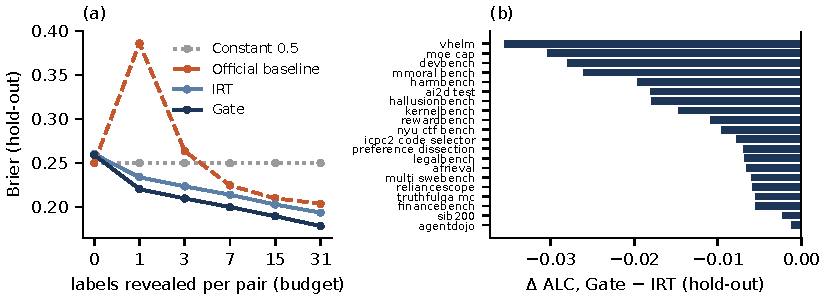
\includegraphics[width=\linewidth]{generated/fig_results.pdf}
\caption{Original generated figure from the shared development study, preserved byte for byte. Left: learning curves on its 20-benchmark hold-out. Right: per-benchmark Gate-minus-IRT ALC differences. The figure describes the hierarchical study in Appendix~\ref{app:shared}, separately from the nine-pair Codabench run in the main text.}
\label{fig:shared-original}
\end{figure}

\paragraph{Why the two model families fit together.}
Rasch--CAIMIRA provides a compact route from a subject's own labels to item-sensitive ability updates. The hierarchical model makes labels useful across related items and subjects within a benchmark. Its development results favor this shared evidence as labels accumulate. The proposed composition in Equation~\ref{eq:extension} asks whether both routes can support the same forecast: a strong initial prediction, a small pair-specific correction, and progressively richer shared structure.

\paragraph{The earlier external comparison.}
Earlier internal development notes also describe a Rasch-plus-rank-2 archive with 384-dimensional lexical features, evaluated on 19 hold-out benchmarks and 1,905 pair-seeds. Those notes report ALC 0.2217 for that archive and 0.2068 for the hierarchical gate, with a benchmark-averaged Gate-minus-external difference of $-0.0139\pm0.0072$. The external model has lower initial Brier score (0.248 versus 0.259), while the gate has lower endpoint Brier score (0.177 versus 0.202). The external model leads on five benchmarks: reliancescope, harmbench, rewardbench, moe\_cap, and preference\_dissection. That comparison also uses different acquisition policies: random for the external model and radius-0.30 for Gate. The observed strengths motivate a combined forecast under matched acquisition.

The earlier comparison omits devbench because byte-identical subject descriptors caused the external model to pool more than 31 labels and raise an error. The selected s44 source likewise matches support by the full subject dictionary and enforces a 31-label limit. An exact archive hash and the pair-level replay records would establish whether the earlier external result belongs to this selected ZIP. That identity remains \textbf{UNVERIFIED}; the figure and tables above characterize the hierarchical study, while the exact-hash component comparison in Table~\ref{tab:local} supplies the selected candidate's local evidence.

\paragraph{Reproduction path and study scope.}
The original \code{make\_numbers.py} reads \code{pairs.csv} and \code{metrics.json} for each run under \code{../runs/}. It computes matched contrasts using subject, benchmark, and seed as keys, averages differences within benchmarks, and forms normal intervals across benchmarks. Its tables, figure, configuration summary, and generation code are included under \code{paper/} in the companion repository. The new compact appendix tables select columns from those same committed rows.

The companion package contains those generated outputs and the script; the underlying raw run files remain outside the package. Full result regeneration and archive identity matching remain separate evidence steps. The development notes record four looks at the hold-out during stack selection and gate weights fitted on an earlier development split. These details bound interpretation while preserving the study's central contribution: shared item structure offers a measurable and interpretable direction for extending sparse adaptation.

\clearpage
\section{Training data, fitting recipe, and release provenance}
\label{app:training}
\paragraph{A completed fit linked to the selected state.}
The CAIMIRA state in submission 1033935 has SHA-256
\begin{center}\small\ttfamily
348088f33fb8080229f5475b95735719a43008a00af8a26b798831a138197eec
\end{center}
An earlier package receipt lists this exact state and binds it to a completed refit and frozen corpus manifest~\citep{release}. That earlier package selected scalar-offset adaptation; submission 1033935 uses the same frozen CAIMIRA state with native two-coordinate adaptation. The state identity transfers the training provenance while each package retains its own prediction policy and results.

\begin{table}[H]
\centering
\caption{Completed CAIMIRA fit recorded in \code{final/refit.json}, linked to the selected state by \code{submission.receipt.json}.}
\small
\begin{tabular}{@{}lr@{}}
\toprule
Quantity & Recorded value \\
\midrule
Training benchmarks / source lineages & 44 / 36 \\
Projected source tables & 176 \\
Input rows / binary response trials & 9,479,991 / 10,951,005 \\
Subject--benchmark pairs & 1,345 \\
Seed / latent dimension & 17 / 2 \\
Optimizer / updates / learning rate & Adam / 300 / 0.01 \\
Final binary cross-entropy & 0.6371165514 \\
Final regularized objective & 0.6637041569 \\
Maximum absolute gradient & $4.6974\times10^{-8}$ \\
Recorded fit time / broader refit command & 24.23 s / 291.98 s \\
\bottomrule
\end{tabular}
\end{table}

\paragraph{Optimization and exported parameters.}
The recovered frozen source weights each subject--benchmark pair equally in the Bernoulli objective and combines repeated outcomes into sufficient statistics. Fitting uses a 384-dimensional lexical map for items and metadata, a learned prior, and subject nuisance abilities shared wherever the serialized subject string repeats. The objective adds ridge with coefficient 0.01, a mean squared nuisance penalty with coefficient 0.5, and CAIMIRA L1 regularization with coefficient $10^{-4}$ over centered difficulties and shifted abilities. Adam uses $(\beta_1,\beta_2)=(0.9,0.999)$, $\epsilon=10^{-8}$, and zero weight decay. Initialization draws CPU float64 Gaussian parameters with scale 0.01, then copies them into the CUDA float32 fit. The exported state retains the learned item heads, metadata prior, centers, and orientation; the subject nuisance table stays outside the deployed predictor. The receipt's field \code{ridge=0.0083239498} is the evaluated penalty contribution, distinct from the coefficient 0.01.

\paragraph{Development protocol.}
The frozen development study records 1,376 trained jobs, 32 evaluated source lineages, and four training-only lineages. It holds out a source lineage, removes training groups whose normalized text matches that lineage, and separates item groups within held pairs. Acquisition histories use seeds 20261030, 20261031, and 20261032; full-donor model seeds are 17, 29, and 1013. The final CAIMIRA refit uses the entire frozen corpus after development. These records describe the development process; the nine-pair formative evaluation and the later 153-pair local replay are separate populations.

\paragraph{Exact reproducibility boundary.}
The public-release package preserves the completed CAIMIRA receipts, source-table digests, and byte-verified fitting source. Its portable runner accepts explicitly normalized data and exports learned state. The original Rasch receipt and full materialized training corpus remain recovery targets. Exact end-to-end regeneration of both submitted state files therefore remains \textbf{UNVERIFIED}. The frozen predictor, score reconstruction, and source-manifest checks are independently executable from the released package.

\clearpage
\subsection{Complete source inventory and data access}
Forty suites use Measurement Data Bank native tables: 31 expanded catalog suites and nine historical mirror admissions, pinned at revision
\begin{center}\small\ttfamily
54074453da7b9911be0f48e4c560be547bc84d21.
\end{center}
Four additional curated supplements are \code{androidworld}, \code{cybench}, \code{mir\_bench}, and \code{swe\_bench\_pro}. The CYBENCH supplement itself draws on the legacy Measurement Data Bank revision \code{589ccfdb8e82}, plus an upstream audit; the complete 40-character revision is preserved in the source registry. Table~\ref{tab:training_sources} names every admitted suite. This inventory describes the verified CAIMIRA corpus; the Rasch receipt gap retains its scope.

\begin{table}[H]
\centering
\caption{All 44 suites in the frozen CAIMIRA training manifest. An asterisk marks a separately curated supplement; the remaining suites use the pinned Measurement Data Bank native tables.}
\label{tab:training_sources}
\small
\begin{tabular}{@{}ll@{}}
\toprule
Benchmark & Benchmark \\
\midrule
\code{abstract\_reason} & \code{matharena} \\
\code{agentdojo} & \code{mathvista\_mini} \\
\code{algotune} & \code{medagentboard} \\
\code{androidworld}$^{*}$ & \code{medhelm\_medcalc\_bench} \\
\code{atmossci\_bench} & \code{mir\_bench}$^{*}$ \\
\code{babilong} & \code{mmlupro} \\
\code{bertaqa} & \code{moe\_cap} \\
\code{brace} & \code{multi\_swebench} \\
\code{cellverse} & \code{radar} \\
\code{clasheval} & \code{real\_webagents} \\
\code{cruxeval} & \code{researchcodebench} \\
\code{cybench}$^{*}$ & \code{statqa} \\
\code{disco} & \code{subjective\_qa} \\
\code{editbench} & \code{swe\_bench\_pro}$^{*}$ \\
\code{fgbench} & \code{swe\_rebench} \\
\code{finegrain\_t2i} & \code{tau2\_bench} \\
\code{goodai\_ltm\_benchmark} & \code{taubench} \\
\code{jetts} & \code{vhelm} \\
\code{kernelbench} & \code{visual\_riddles} \\
\code{lexeval} & \code{wonderbread} \\
\code{liveaopsbench} & \code{workarena} \\
\code{llm\_uncertainty\_bench} & \code{worldcentralbanks} \\
\bottomrule
\end{tabular}
\end{table}


\paragraph{Source identities and permitted access.}
The companion \code{data/sources/} directory supplies \code{DATA\_SOURCES.csv}, upstream locations and revisions, source-specific rights information, and a retrieval manifest. The frozen projected table inventory records SHA-256 for all 176 files: \code{facts}, \code{items}, \code{subjects}, and \code{ungraded} for each suite. The bundled source records distinguish these derived tables from the upstream data and preserve the transformation's provenance. A local table verifier checks supplied corpus files against the frozen digests.

Measurement Data Bank's CC BY-SA 4.0 terms apply to its curation; underlying sources retain their own licenses and access conditions~\citep{measurementdb2026}. The release therefore includes derived result tables, manifests, learned states, and code, with upstream retrieval instructions for source data. Source-specific rights and availability govern redistribution of the remaining corpus. Completing the permitted supplemental-data release remains part of the presentation release record.

\paragraph{Additional model and assistance disclosure.}
The selected Rasch--CAIMIRA runtime uses deterministic lexical hashing and its bundled learned coefficients. It uses local computation without a pretrained text encoder or a model-provider API. The separately discussed hierarchical extension has its own 180-benchmark build inventory in \code{extensions/gate/build\_info.json}; the earlier study's evaluation fit used 160 training benchmarks and 20 held-out benchmarks. These inventories remain separate from the selected CAIMIRA fit. ChatGPT and Claude Code assistance is disclosed with the references.

\end{document}
